\documentclass{article}
\usepackage[utf8]{inputenc}
\usepackage{algorithm}
\usepackage{algorithmicx}
\usepackage{algcompatible}
\usepackage{amsmath}
\usepackage{amssymb}
\usepackage{wrapfig}
\usepackage{graphicx}
\usepackage{geometry}
\geometry{margin=1in}


\title{CS 509 Lab Assignment 1}
\author{ISHAN TRIPATHI 2021AIM1009}
\date{Feb 2021}
\DeclareUnicodeCharacter{2212}{-}

\begin{document}
\maketitle

\section{Introduction}
The problem of path finding in road networks has been of great importance. Its value addition potential gets boosted even further when the path-finding algorithms start to consider the traffic congestion patterns. A recent report from McKinsey \cite{gunturi2015critical} estimates that we can save billions of dollars (annually) by helping vehicles avoid traffic congestion. \par
Given the overall significance of the problem area, several researchers (e.g., \cite{davidson2014work, demiryurek2010case}) have been exploring it from different aspects. Among these, the most fundamental being: computing the fastest path between a source and destination for a given departure-time (at source). In this problem, the underlying road network (and its time-varying traffic congestion) is conceptualized as a time varying graph (more details later). Given a time-varying graph representation of the road network, a source $s$ , a destination $d$ and, a departure-time $(t_{dep})$; the goal is to determine a journey $\mathcal{L}$ between $s$ and $d$ which departs from $s$ at time $t_{dep}$. The key property of $\mathcal{L}$ being that there does not exist any other journey $\mathcal{L'}$ between $s$ and $d$ which departs from $s$ at time $t_{dep}$ but arrives at destination earlier than $\mathcal{L}$. This optimal journey $\mathcal{L}$ has been referred to as a shortest lagrangian path in some literature \cite{demiryurek2010case} (more details later).
\\*
\\*
\textbf{Limitations of the Related Work:} Though there have been several works in the area of parallel algorithms
for the shortest paths problem (e.g., \cite{maleki2016dsmr, simmhan2015distributed, analytics2016age,chakaravarthy2016scalable}), they cannot be extended for our SLP problem because they
cannot be modified to follow the “Lagrangian reference frame”. Parallel algorithms \cite{analytics2016age, chakaravarthy2016scalable} based on label
correcting based approaches are in principle \emph{not suitable} for implementing Lagrangian reference frame.

\section{Problem Statement}
We now formally define the problem of capacity constrained assignment (CCA) by detailing the input, output and the objective function:\\
\textbf{Given:}
\begin{itemize}
    \item A road network represented as a directed $G(V, E)$, where each edge $e \in E$ has a positive cost.
    \item A set of service centers ${S = \{s_1, ..., s_{n_s}\}}$ where $S \subset V$. Each service center ${s_i}$ has a capacity ${c_{s_i}}$ and a penalty function ${p_{s_i}}$.
    \item A set of demand vertices $D = \{d_1, ..., d_{n_d}\}$ where $D \subset V - S$.
\end{itemize}

\begin{flushleft}
\textbf{Output:} An allotment consisting of pairs $< d_k, s_j >$.
\\
\textbf{Objective Function:}
\end{flushleft}


\[
\textbf{$Min$} 
\Bigg \{ 
    \sum_{\substack{\text{$s_i \in$ Service} \\ \text{Centres}}} 
    \Bigg \{ 
        \sum_{\substack{\text{$d_j \in$ Demand~vertices} \\ \text{allotted~to~$s_i$}}} SCost(d_j, s_i) 
    \Bigg \}
    ~~~+~~~Total~~~Penalty~~~across~~~all~~~s_i 
\Bigg \}
\tag{1}
\]




% \begin{equation}
% \textbf{Min} \left \{ \left \{ \sum_{s_i \in Service Centres} \right \}\left \{ \sum_{\substack{\text{d_j \in Demand~vertices} \\ \text{alloted~to~s_i}}} SCost(d_j, s_i) \right \} + Total~~Penalty~~across~~all~~s_i \right \}
% \end{equation}


% \begin{equation}
% \sum

% \end{equation}  

% \emph{\textbf{Min}} \sum_{s_i ~ belongs ~ to ~ Service \\ ~ Centers} \sum_{Demand ~ vertices ~ allotted ~ to ~ s_i}^{}  SCost ~ (d_j, s_i) ~ + ~ Total ~ penalty ~ across ~ all ~ s_i 


% % x_i^p = \sum_{k=1}^{\infty} \sum_{j=1}^{N} \gamma^k (A^k)_{ji} \beta~\alpha~\omega
% \begin{split}
    
% \emph{\textbf{Min}} \sum_{s_i ~ belongs ~ to ~ Service \\ ~ Centers} \sum_{Demand ~ vertices ~ allotted ~ to ~ s_i}^{}  SCost ~ (d_j, s_i) ~ + ~ Total ~ penalty ~ across ~ all ~ s_i 
% \end{split}
% \label{prob_eqn}


\section{Sample Equations}


\begin{align*}
E_{sys} (t) &= E^{comm}_{edge} (t) + E^{hover}_{edge} (t) + \Bigg( \sum_{i=1}^{N} ( E_{i}^{comm} (t) ) \Bigg) \\
&= \kappa * \|{vel (t)}\|^2
\\
&= ( 2^{\frac{D_{edge}}{W}} - 1) * \frac{N_0 W}{\alpha}
\tag{2}
\end{align*}


% \[ \sum_{n=1}^{\infty} 2^{-n} = 1 \]


\section{Overview of solution}

\begin{wrapfigure}{r}{0.55\textwidth}
  \begin{center}
    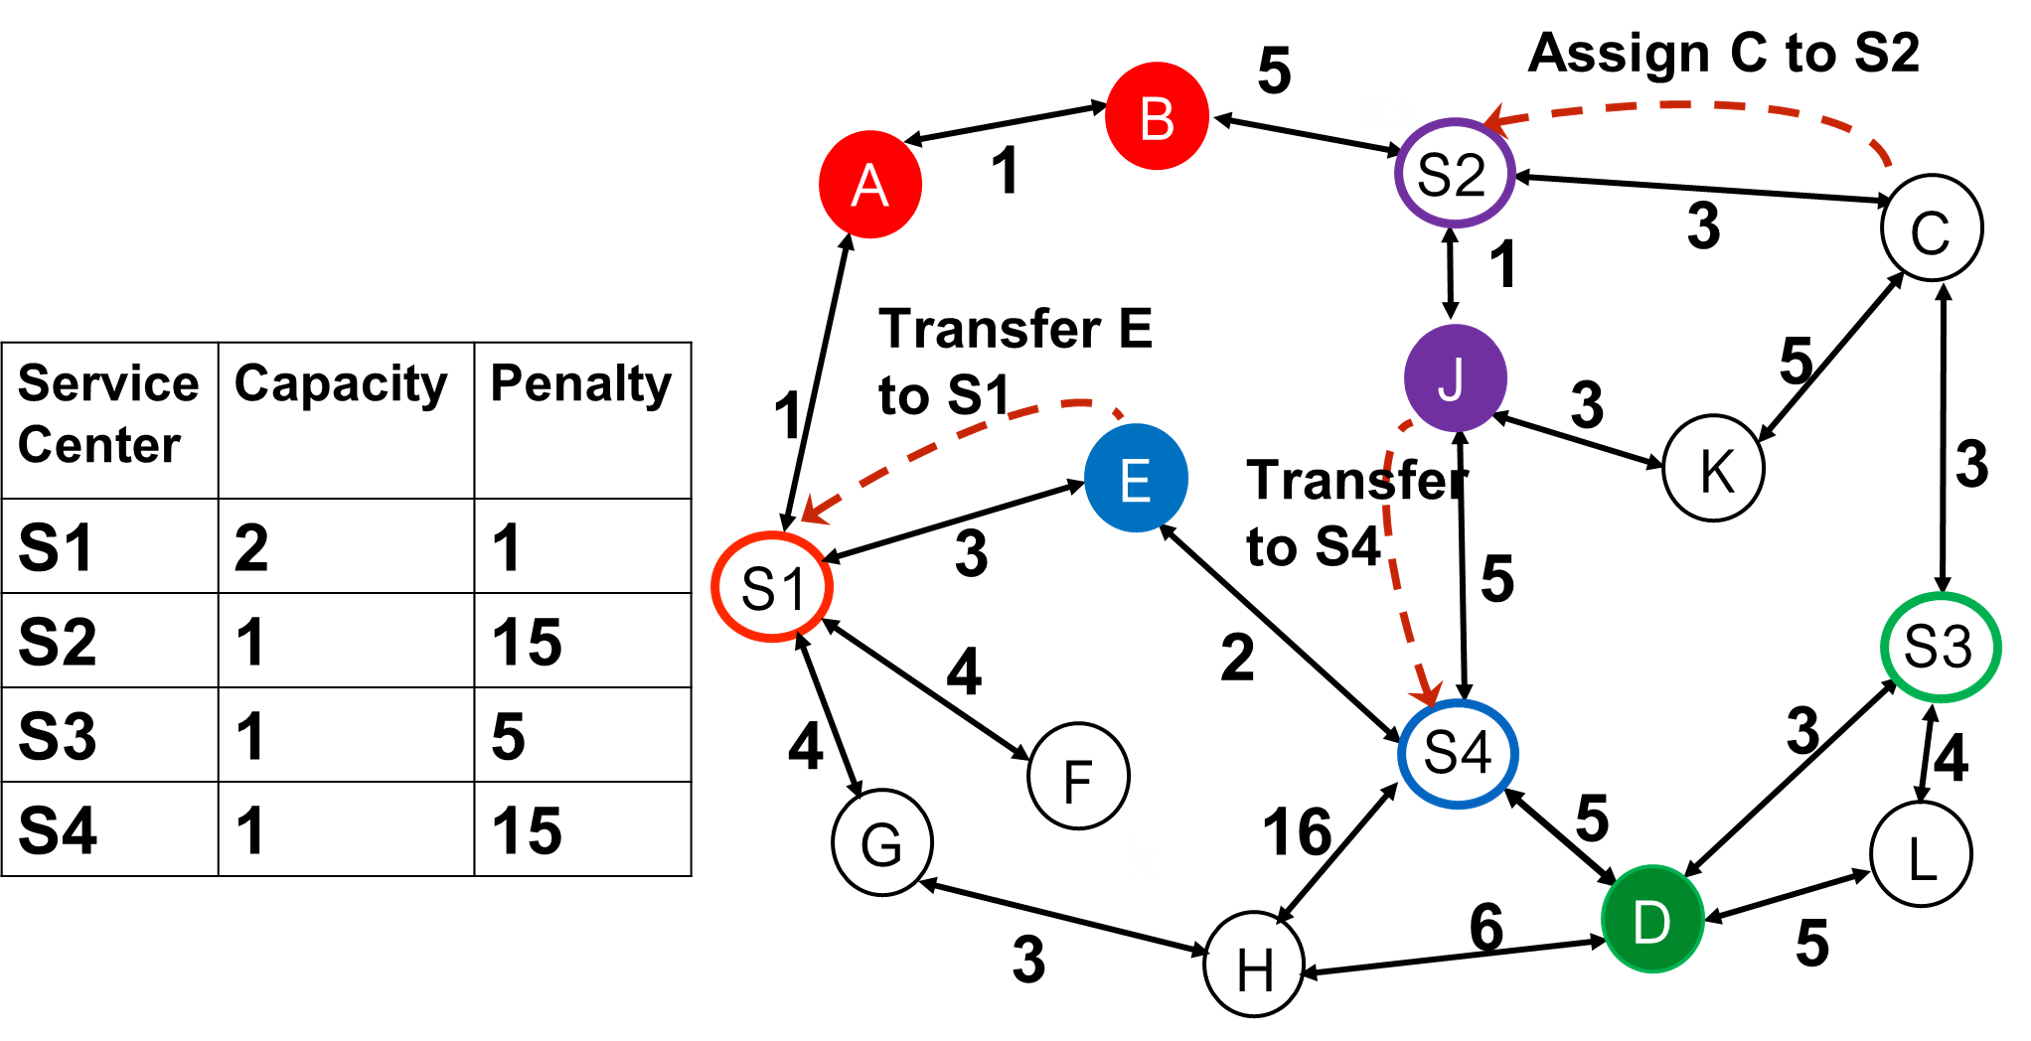
\includegraphics[width=0.48\textwidth]{run_eg_one.png}
  \end{center}
  \caption{Figure 1: A partially constructed assignment on a sample input. Processed demand nodes are filled with the same color as their respective service center. (Best in color)}
\end{wrapfigure}


This assignment could have happened under following two cases: \textbf{Case (a)} $s_i$ had free space (in terms of capacity) or; \textbf{Case (b)} $s_i$ was already full. Case (a) is quite straightforward and no further operations are needed. Note that in this case, we also need not pay any penalty for this assignment. However, in case(b), after assigning $d_i$ to $s_j$ , the algorithm undertakes the process of re-organizing the current solution with an intention of lowering the current objective function value. Note that in case (b), the objective function would increase by the quantity $\delta = SCost(d_i, s_j ) + Penalty(s_i)$ after the assigning $d_i$ to $s_j$. We now briefly present our idea of re-organization at high level.


\begin{algorithm}[h]
\caption{Assignment Subspace Re-organization based Approach for CCA}
\textbf{Input:} (a) $\alpha:$ allowed breadth of the search in assignment subspace tree ($\alpha \leq {\mid S \mid} − 1$);
\\
\textbf{Output:} Assignment $\mathcal{A}$ with objective function value $\Delta$
\begin{algorithmic}[1]
\WHILE{$ ClosestSC$ heap is not empty}
\IF {$s*$ has vacancy}
\STATE {Decrement capacity of $s*$}
\ELSE 
\STATE {Increment $\Delta$  by penalty corresponding to $s*$}
\STATE {Initialize the list of seeds $\Gamma$}
\STATE {$\Gamma$ ← Determine $\alpha$ seeds}
\IF {$\alpha \leq \tau$ } /*allowed breadth of the search is less than \#threads*/
\STATE {$\lambda$ ← Create $\alpha$ threads}
\ELSE /*allowed breadth of the search is more than threads*/
\STATE {$\lambda$ ← Create $\tau$ threads}
\ENDIF
\STATE {Create a job queue $JQ$ with seeds present in $\Gamma$. /*Each seed is a job*/}
\STATE {Barrier to ensure that all threads in $\Lambda$ terminate}
\ENDIF
\ENDWHILE
\end{algorithmic}
\end{algorithm}

\bibliographystyle{plain}
\bibliography{citations}


\end{document}